\documentclass[tikz,border=8pt]{standalone}
\usepackage{amsmath,amssymb}
\usepackage{tikz}
\usetikzlibrary{positioning,fit,arrows.meta,calc}

\newcommand{\Dtot}{D_{\mathrm{tot}}}
\newcommand{\Dfar}{D'}
\newcommand{\Dloc}{D}
\newcommand{\rep}{\mathrm{rep}}

\begin{document}
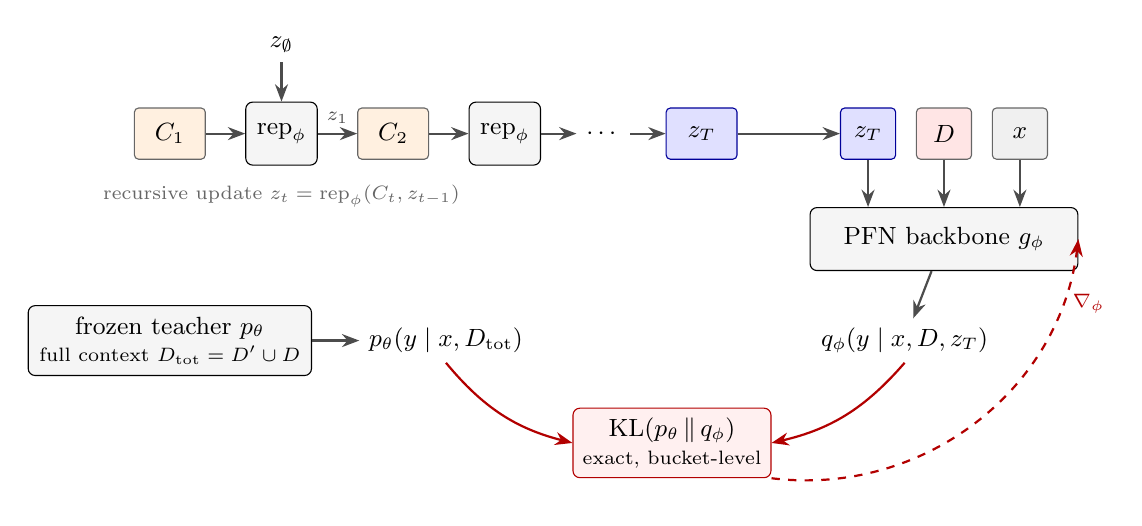
\begin{tikzpicture}[
  font=\small,
  chunk/.style={draw=black!60, fill=orange!12, rounded corners=1.5pt,
    minimum width=9mm, minimum height=6.5mm, inner sep=1.5pt},
  ztok/.style={draw=blue!60!black, fill=blue!12, rounded corners=1.5pt,
    minimum width=9mm, minimum height=6.5mm, inner sep=1.5pt},
  module/.style={draw=black, fill=black!4, rounded corners=2.5pt,
    minimum height=8mm, inner sep=4pt, align=center},
  loss/.style={draw=red!70!black, fill=red!6, rounded corners=2.5pt,
    minimum height=7mm, inner sep=3.5pt, align=center},
  arr/.style={-{Stealth[length=2.2mm]}, thick, black!70},
]
\node[chunk] (c1) {$C_1$};
\node[module, right=5mm of c1] (rep1) {$\rep_\phi$};
\node[chunk, right=5mm of rep1] (c2) {$C_2$};
\node[module, right=5mm of c2] (rep2) {$\rep_\phi$};
\node[right=4.5mm of rep2] (dots) {$\cdots$};
\node[ztok, right=4.5mm of dots] (zT) {$z_T$};
\node[above=5mm of rep1] (z0) {$z_\emptyset$};
\draw[arr] (z0) -- (rep1);
\draw[arr] (c1) -- (rep1);
\draw[arr] (rep1) -- node[above, font=\scriptsize] {$z_1$} (c2.west |- rep1.east);
\draw[arr] (c2) -- (rep2);
\draw[arr] (rep2) -- (dots);
\draw[arr] (dots) -- (zT);
\node[below=1.2mm of rep1.south, font=\scriptsize, black!60] {recursive update
  $z_t = \rep_\phi(C_t, z_{t-1})$};

\node[ztok, right=13mm of zT, minimum width=7mm] (zin) {$z_T$};
\node[chunk, fill=red!10, right=2.5mm of zin, minimum width=7mm] (dloc) {$\Dloc$};
\node[chunk, fill=black!6, right=2.5mm of dloc, minimum width=7mm] (xq) {$x$};
\node[module, below=6mm of dloc, minimum width=34mm] (backbone)
  {PFN backbone $g_\phi$};
\draw[arr] (zT) -- (zin);
\draw[arr] (zin.south) -- (backbone.north -| zin.south);
\draw[arr] (dloc.south) -- (backbone.north -| dloc.south);
\draw[arr] (xq.south) -- (backbone.north -| xq.south);
\node[below=6mm of backbone, xshift=-5mm, align=center] (q)
  {$q_\phi(y \mid x, \Dloc, z_T)$};
\draw[arr] (backbone) -- (q);

\node[module, align=center] (teacher) at (c1 |- q)
  {frozen teacher $p_\theta$\\[-1pt]{\scriptsize full context $\Dtot = \Dfar \cup \Dloc$}};
\node[right=6mm of teacher, align=center] (p) {$p_\theta(y \mid x, \Dtot)$};
\draw[arr] (teacher) -- (p);
\node[loss] (kl) at ($($(p.east)!0.5!(q.west)$)+(0,-13mm)$)
  {$\mathrm{KL}(p_\theta \,\Vert\, q_\phi)$\\[-1pt]{\scriptsize exact, bucket-level}};
\draw[arr, red!70!black] (p.south) to[bend right=18] (kl.west);
\draw[arr, red!70!black] (q.south) to[bend left=18] (kl.east);
\draw[arr, red!70!black, dashed] (kl.south east) to[bend right=45]
  node[right, pos=0.85, font=\scriptsize, red!70!black] {$\nabla_\phi$}
  (backbone.east);
\end{tikzpicture}
\end{document}
